\begin{figure}[htp]
	\begin{center}
	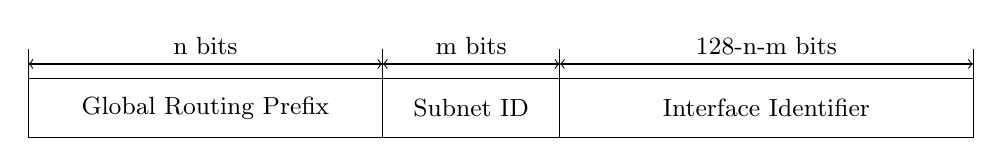
\begin{tikzpicture}[scale=0.75]
		\draw (0,0) rectangle (16,1);
		\draw (0,1) -- ++(0,0.5);
		\draw (6,0) -- ++(0,1.5);
		\draw (9,0) -- ++(0,1.5);
		\draw (16,1) -- ++(0,0.5);
		\node at (3, 0.5) {\small Global Routing Prefix};
		\node at (7.5, 0.5) {\small Subnet ID};
		\node at (12.5, 0.5) {\small Interface Identifier};
		\draw[<->] (0,1.25) -- (6,1.25) node[midway, above] {\small n bits};
		\draw[<->] (6,1.25) -- (9,1.25) node[midway, above] {\small m bits};
		\draw[<->] (9,1.25) -- (16,1.25) node[midway, above] {\small 128-n-m bits};
	\end{tikzpicture}
	\end{center}
	\caption{Global Unicast address}
	\label{fig:ipv6_global_unicast}
\end{figure}